\documentclass[border=0.2cm]{standalone}
\usepackage{tikz}
\usetikzlibrary{automata, arrows.meta, positioning}

\begin{document}

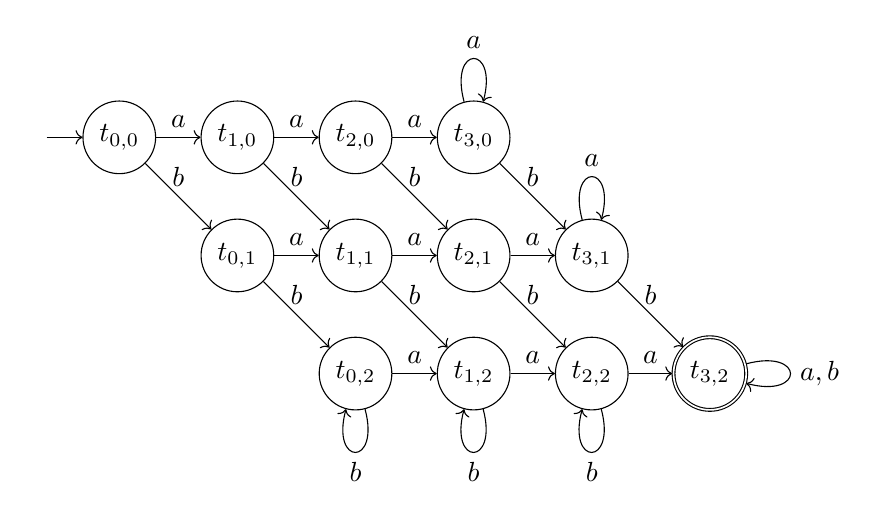
\begin{tikzpicture} [
    every initial by arrow/.style = {-To},
    every loop/.style = {-To}]
    \node (t00) [state, initial, 
        initial text={}] at (0,0) {$t_{0,0}$};
    \node (t10) [state] at (1.5,0) {$t_{1,0}$};
    \node (t20) [state] at (3,0) {$t_{2,0}$};
    \node (t30) [state] at (4.5,0) {$t_{3,0}$};

    \node (t01) [state] at (1.5,-1.5) {$t_{0,1}$};
    \node (t11) [state] at (3,-1.5) {$t_{1,1}$};
    \node (t21) [state] at (4.5,-1.5) {$t_{2,1}$};
    \node (t31) [state] at (6,-1.5) {$t_{3,1}$};

    \node (t02) [state] at (3,-3) {$t_{0,2}$};
    \node (t12) [state] at (4.5,-3) {$t_{1,2}$};
    \node (t22) [state] at (6,-3) {$t_{2,2}$};
    \node (t32) [state, accepting] at (7.5,-3) {$t_{3,2}$};
    
    \path [-To]
        (t00) edge node [above] {$a$} (t10)
        (t10) edge node [above] {$a$} (t20)
        (t20) edge node [above] {$a$} (t30)
        (t30) edge [loop above] node {$a$} ()

        (t00) edge node [above] {$b$} (t01)
        (t10) edge node [above] {$b$} (t11)
        (t20) edge node [above] {$b$} (t21)
        (t30) edge node [above] {$b$} (t31)

        (t01) edge node [above] {$a$} (t11)
        (t11) edge node [above] {$a$} (t21)
        (t21) edge node [above] {$a$} (t31)
        (t31) edge [loop above] node {$a$} ()

        (t01) edge node [above] {$b$} (t02)
        (t11) edge node [above] {$b$} (t12)
        (t21) edge node [above] {$b$} (t22)
        (t31) edge node [above] {$b$} (t32)

        (t02) edge node [above] {$a$} (t12)
        (t12) edge node [above] {$a$} (t22)
        (t22) edge node [above] {$a$} (t32)
        (t32) edge [loop right] node {$a,b$} ()

        (t02) edge [loop below] node {$b$} ()
        (t12) edge [loop below] node {$b$} ()
        (t22) edge [loop below] node {$b$} ();


    %     (q0) edge node [above] {$b$} (q1)
    %     (q1) edge node [above] {$b$} (q2)
    %     (q0) edge [loop above] node {$a$} ()
    %     (q1) edge [loop above] node {$a$} ()
    %     (q2) edge [loop above] node {$a,b$} ();
\end{tikzpicture}

\end{document}